\subsection{Prueba de aceptación} \label{Cuestionario}
Esta prueba está basada en modelo de pruebas \textit{Game Flow}\cite{gameflow}.
\textit{Game Flow} utiliza estrategias heurísticas de usabilidad y experiencia
de usuario para medir el nivel de aceptación de los usuarios. Este modelo permite
medir varios aspectos de los cuales en este proyecto se probarán:
{\it enjoyment}(disfrute), diseño de interfaces, mecánicas y jugabilidad.
\\
\par
Se toma la decisión de aplicar las pruebas \textit{Game Flow} por nivel ya que en
caso de realizar modificaciones para mejorar la experiencia de usuario estos
cambios se podrán orientar a un nivel en especifico si al final de las pruebas
un nivel en específico genera problemas entre los usuarios por su elevada
dificultad o facilidad. Por otra parte aplicar las pruebas por niveles permite que los jugadores no tengan que jugar todo el videojuego para tener que responder la encuesta lo que traduce en que las pruebas no tomarán mucho del tiempo de los participantes.
\\
\par
Esta prueba de aceptación se dividió en dos partes:
\begin{itemize}
    \item \textbf{Presencial}: Esta prueba se realiza sobre la población de la
    Escuela Superior de Cómputo(ESCOM) del Instituto Politécnico Nacional(IPN).   
    \item \textbf{En línea:} Para esta prueba se publicaron los \textit{links} del
    archivo APK y de la encuesta en foros de desarrollo de videojuegos y grupos
    de \textit{FaceBook} con la misma temática.
\end{itemize}
 
\subsubsection{Objetivo}
Evaluar el nivel de aceptación de juego entre los jugadores y obtener la opinión
de los mismos sobre posibles mejoras al juego.

\subsubsection{Herramientas}
Para aplicar ambos tipos de pruebas se utilizaron:
    \begin{itemize}
        \item \textbf{Archivo APK del juego:} Este archivo fue proporcionado por
        medio de un \textit{link} y por medio de transferencia de archivos al teléfono
        de los encuestados desde una computadora.
        \item \textbf{Cuestionario:} El cuestionario fue proporcionado desde un
        \textit{link} empleando la herramienta de \textit{Google Docs} para agilizar
        el conteo de los resultados.   
    \end{itemize}

\subsubsection{Aplicación}
Para la aplicación de las pruebas en línea se distribuyen los links del archivo APK y del cuestionario en diferentes foros de desarrolladores y grupos de \textit{Facebook}. En algunos casos diferentes usuarios ofrecieron retroalimentación del juego en los comentarios de la publicación o enviando mensajes privados.
\\
\par
En el caso de las pruebas presenciales, se solicita a diferentes profesores del
plantel de la ESCOM. En cada uno de los grupos en los que se aplica la encuesta
se da una presentación del argumento del juego y su objetivo. Después se dan las
instrucciones de la prueba, los \textit{link} a los archivos y al cuestionario y
se indica el nivel a probar. Además de la encuesta se puede observar las
reacciones de lo jugadores mientras prueban el juego
(ver figura \ref{fig:AlumnosESCOM}).

\begin{figure}
  \centering
 
   \subfigure[Dos alumnos de la Escuela Superior de Cómputo probando el juego.] {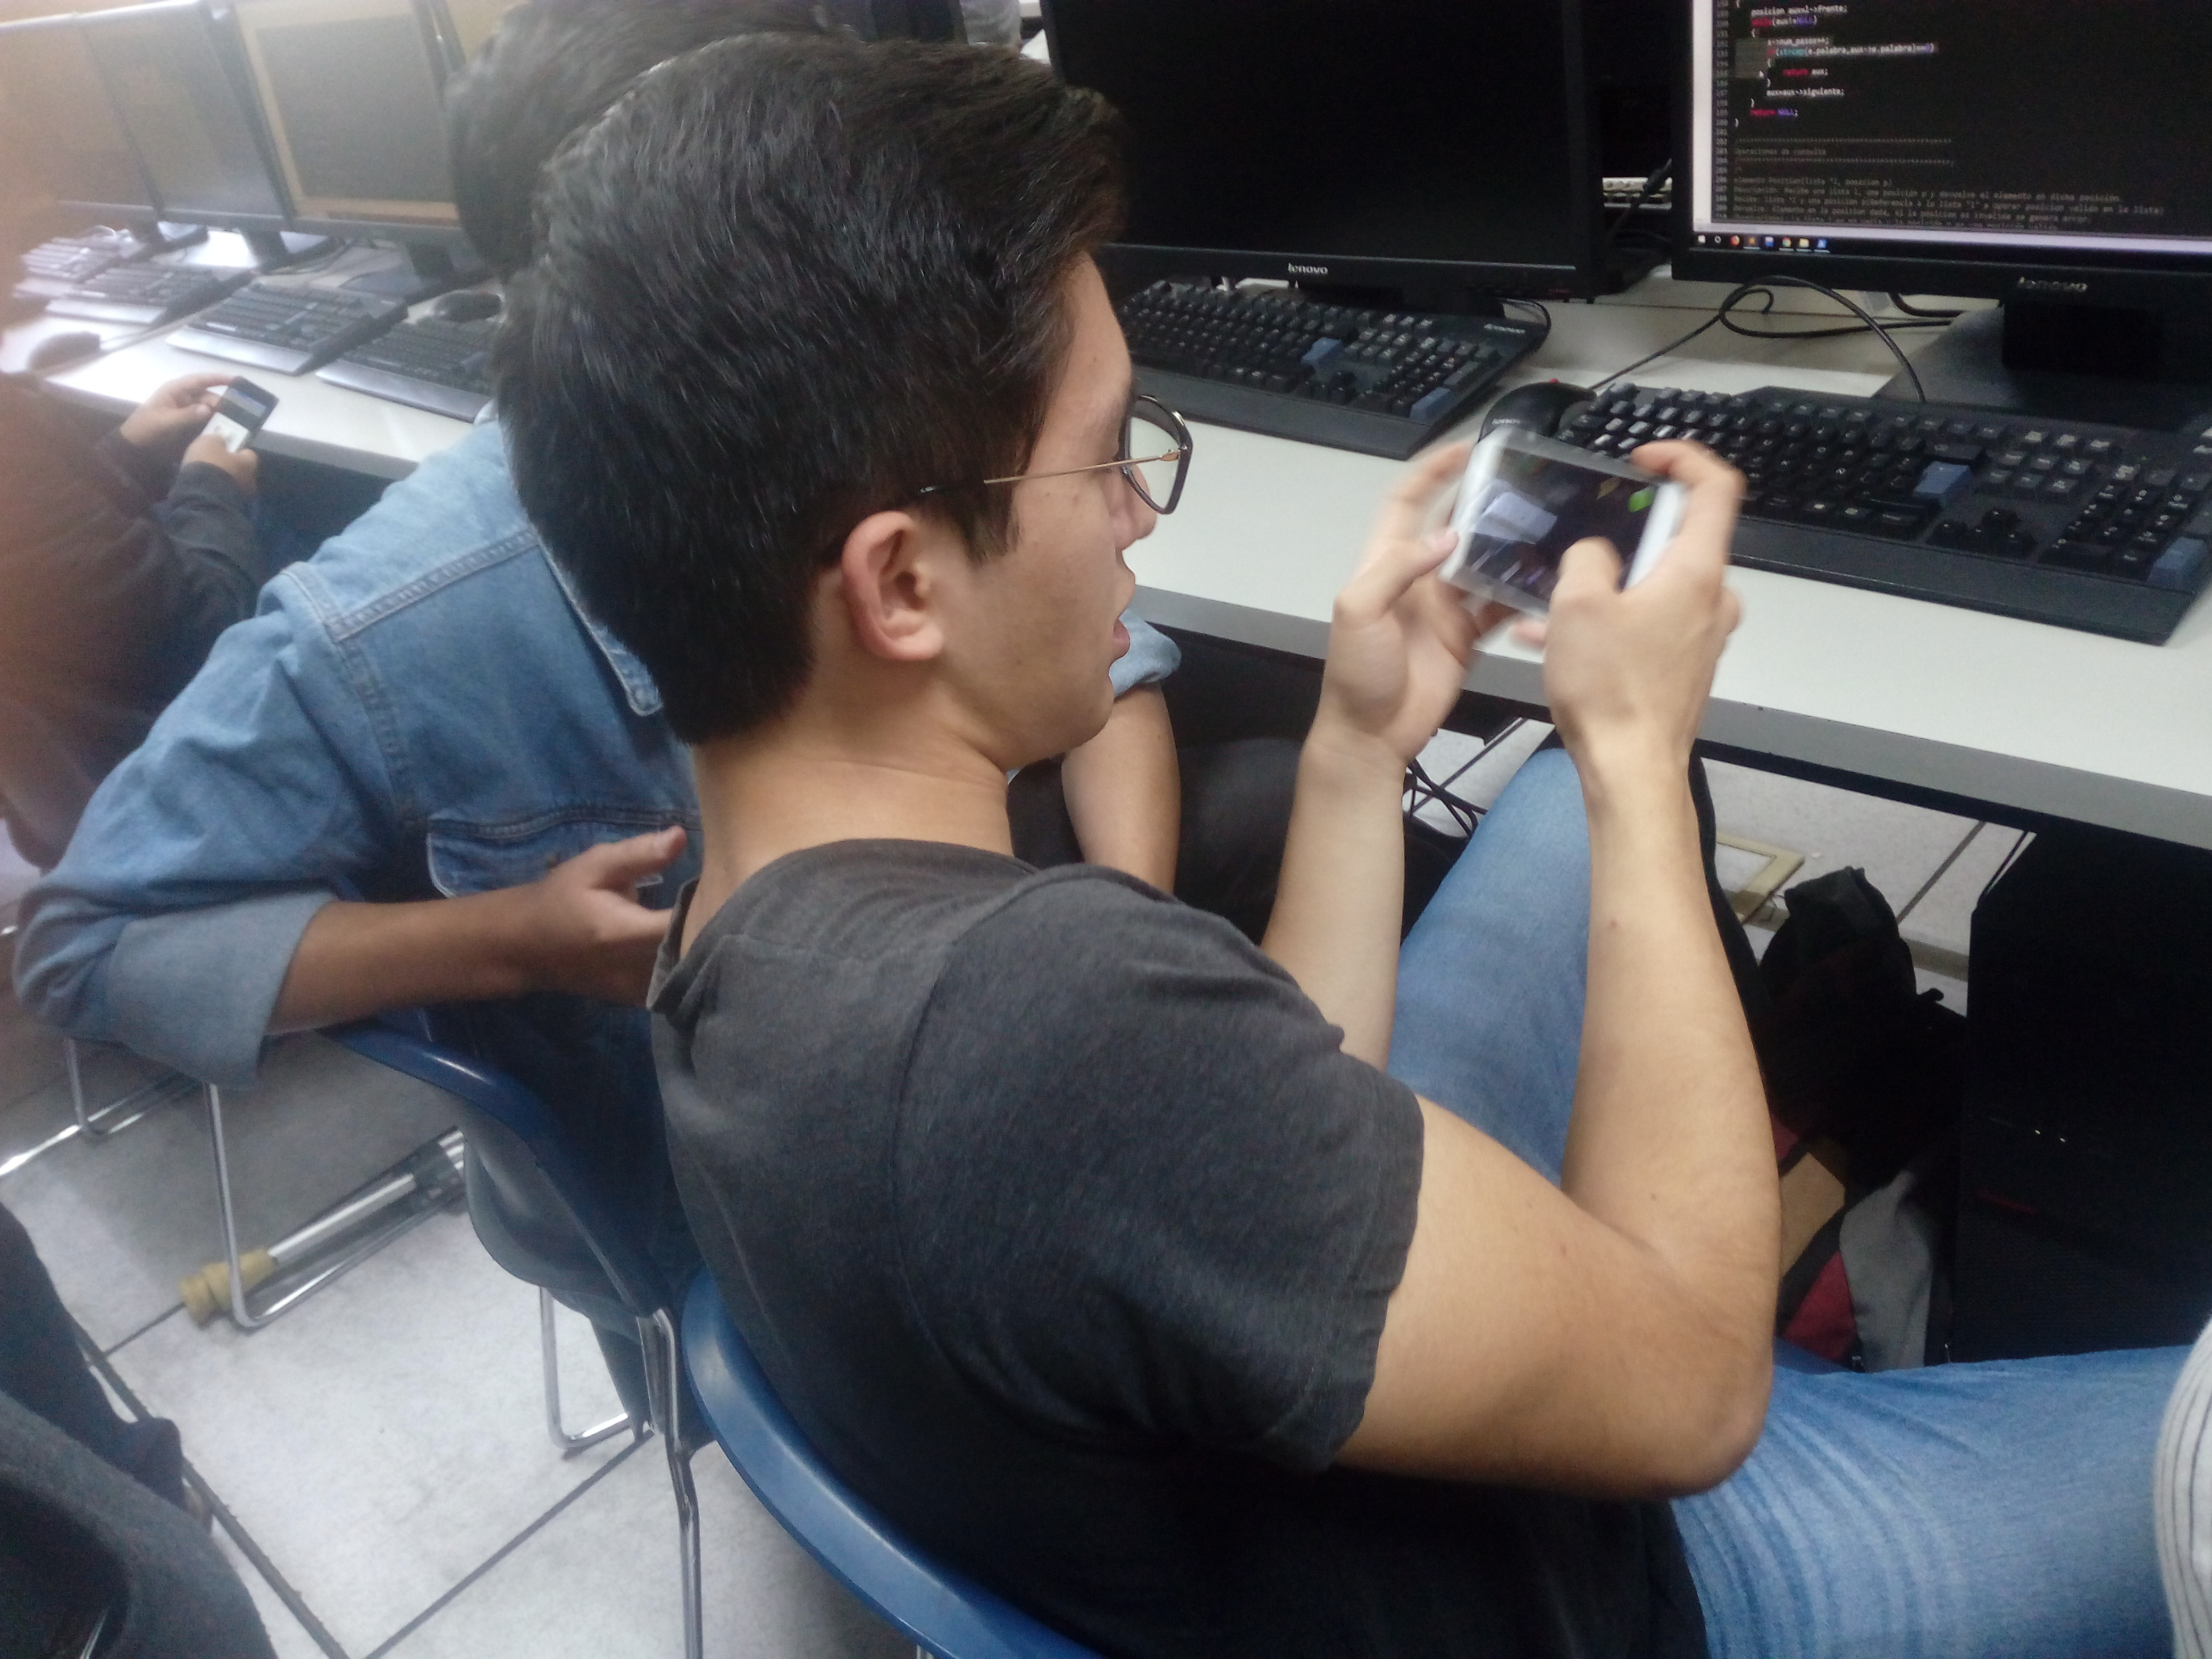
\includegraphics[width=0.4 \textwidth]
   {04ResultadosObetnidos/imagenes/usuarios01}}
        
        \subfigure[Grupo de alumnos de la Escuela Superior de Cómputo probando el
        juego.] {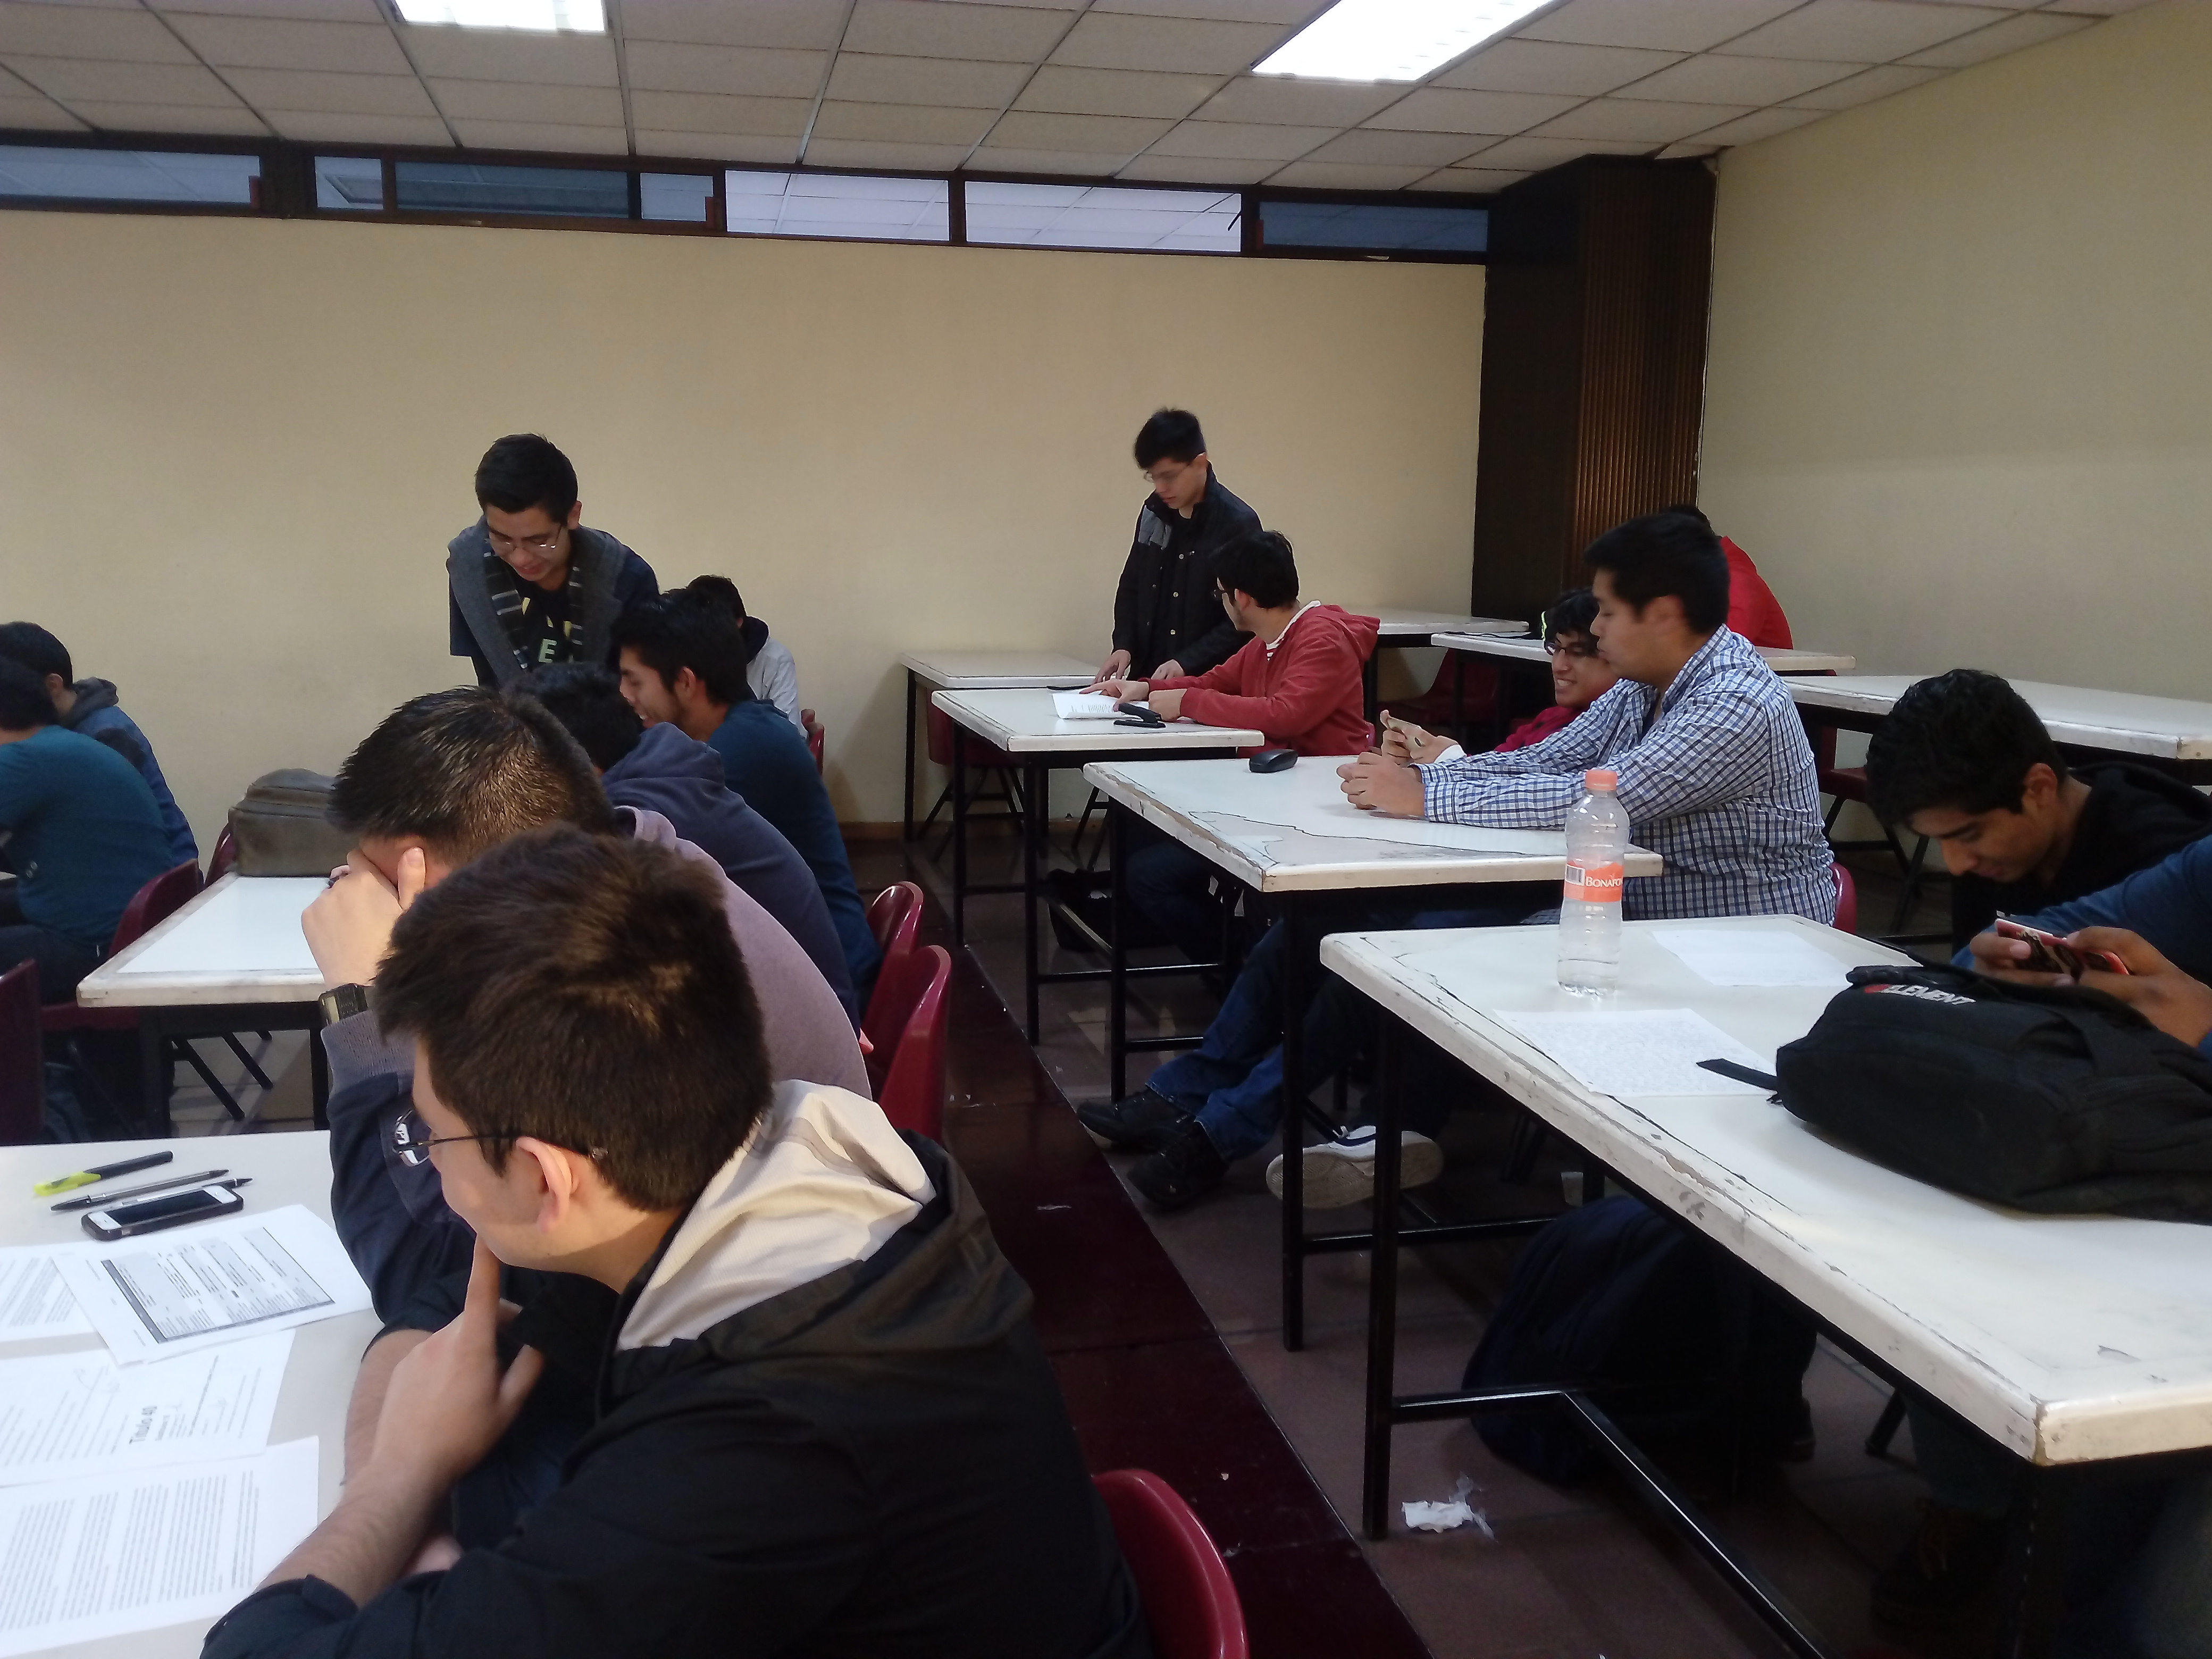
\includegraphics[width=0.4 \textwidth]{04ResultadosObetnidos/imagenes/usuarios02}}
  \caption{Resultados de la herramienta \textit{profiler} al analizar una cinemática.}
  \label{fig:AlumnosESCOM}
\end{figure}

\subsubsection{Resultados}
A continuación se presentan algunos de los resultados de la encuesta,
lo resultados completos se encuentran en el anexo \ref{Anexo:resultados}.
\begin{itemize}
        \item La principal marca de dispositivos con el que fue probado el juego fue
        Motorola con sistema operativo Android 7.
        \item La mayoría de los usuarios consideran como bueno el movimiento del
        personaje.
        \item La mayoría de los usuarios consideran que la respuesta de la
        \textit{GUI} es buena.
        \item La mayoría de los usuarios opina que la actualización de la barra de
        tonali es buena pero les gustaría que existiera un indicador numérico para ver
        la cantidad de disparos que les queda.
        \item La mayoría de los usuarios considera que lo hace hace débil a un personaje
        es su patrón de movimiento y no la cantidad de daño que pueda generar; por
        otro lado también la mayoría de los usuarios considera que lo que hace a un
        enemigo fuerte es su patrón de movimiento.
        \item El Fantasma morado es considerado por muchos usuarios como el enemigo más
        poderoso en los niveles de plataforma.
        \item El fantasma rojo es considerado por muchos usuarios como el enemigo más
        débil en los niveles de plataforma.
        \item Las dos principales causas de muerte en los jugadores son el tiempo
        de respuesta de la \textit{GUI} y que los enemigos eran demasiado fuertes.
\end{itemize}

Adicionalmente lo jugadores hicieron observaciones y peticiones que ellos
consideran podrían mejorar la experiencia de juego:
\begin{itemize}
        \item Animación que indique que un enemigo ha recibido daño.
        \item Barra de vida para los enemigos.
        \item Posibilidad de que el jugador se agache.
        \item Mensajes de confirmación para los botones que llevan al menú de selección
        y que cierran la aplicación.
        \item Mejorar el comportamiento de los disparos.
\end{itemize}

\subsubsection{Conclusiones}
Las conclusiones que se obtuvieron de las pruebas son:
    \begin{itemize}
        \item Hacer el salto más estable mejorará la experiencia del jugador.
        \item Mejorar el tiempo de respuesta de la GUI y agregar una animación
        que indique que un botón ha sido oprimido mejorará la experiencia del
        jugador ya que la mayoría de los usuarios indica que este aspecto fue la
        causa de la mayoría de sus muertes dentro del juego.
        \item Si se desea hacer niveles de plataforma más difíciles estos deben
        de contener más enemigos normales de tipo Fantasma Morado ya que estos son
        los que la mayoría de los jugadores consideran como el más fuerte.
        \item Si se desea hacer niveles de plataforma más fáciles estos deben
        de contener más enemigos normales de tipo Fantasma Rojo ya que estos son los
        que la mayoría de los jugadores consideran como el más débil.
    \end{itemize}